%\vspace*{-2mm}
\begin{figure}[!htb] 
\begin{center}
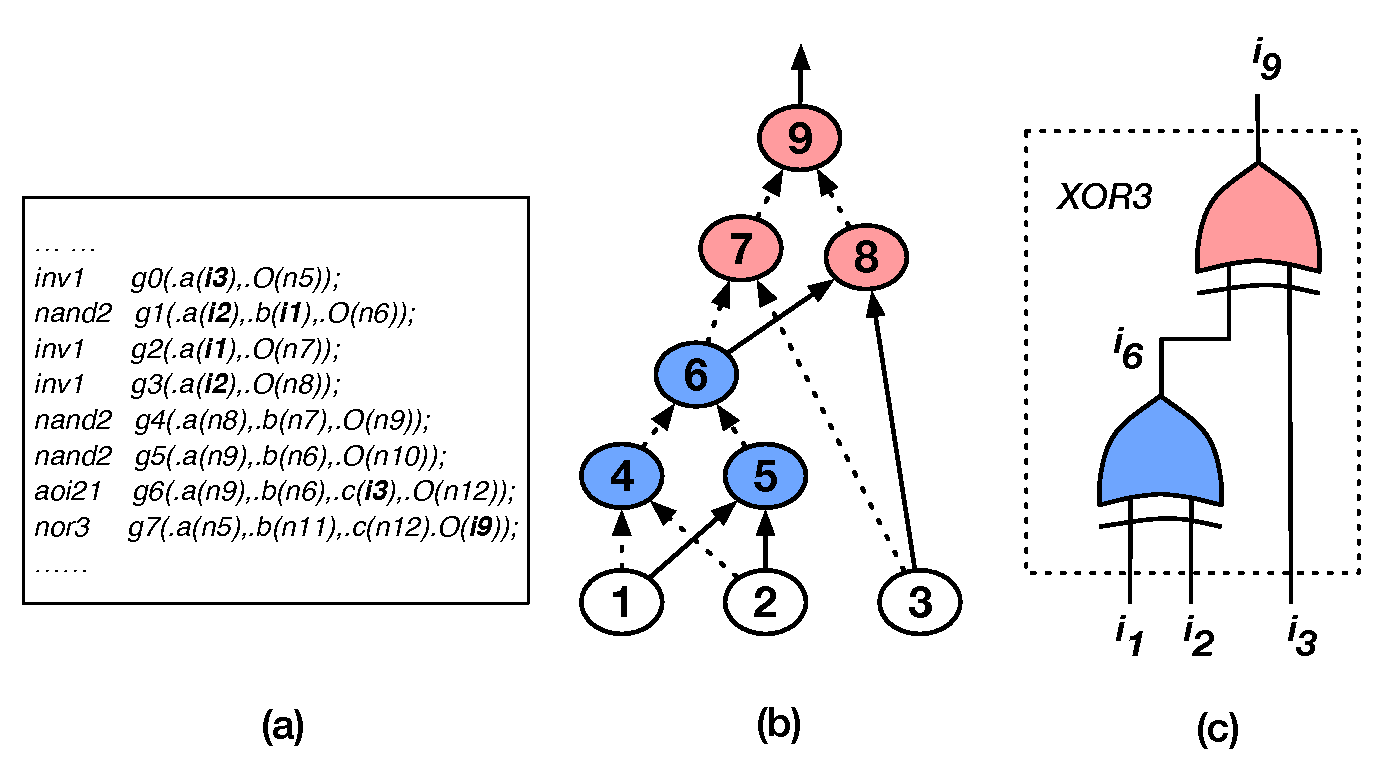
\includegraphics[scale=0.35]{../figs/aig-xor3.eps}
\caption{a) Post-synthesized XOR3 gate-level netlist. b) AIG of the synthesized XOR3 gate-level netlist. (c) The extracted two XOR2 functions (nodes 6 and 9) and one XOR3 function (node 9).}
\label{fig:xor3-aig}
\end{center}
\end{figure}

\section{Background} \label{sec:related-work}
%\vspace*{-2mm}

\subsection{Formal Verification of Arithmetic Circuits}
Verification of arithmetic circuits is performed using a variation of \textit{combinational equivalence checking} (CEC) referred to as \textit{arithmetic combinational equivalence checking} (ACEC) \cite{sayedformal:date-2016}. Several approaches have been applied to equivalence check an arithmetic circuit against its functional specification, including \textit{canonical diagrams}, \textit{satisfiability} theories, \textit{theorem proving}, etc. Different variants of canonical, graph-based representations have been proposed, including Binary Decision Diagrams (BDDs) \cite{bryant:1986-bdd}, Binary Moment Diagrams (BMDs) \cite{bmd95} \cite{bryant:tr97}, Taylor Expansion Diagrams (TED) \cite{ted:tcomp06}, and other hybrid diagrams.
%
While BDDs have been used extensively in logic synthesis, their application to verification of arithmetic circuits is limited by the prohibitively high memory requirements for complex arithmetic circuits, such as multipliers. 
Boolean satisfiability (SAT) and satisfiability modulo theories (SMT) solvers have also been applied to solve ACEC problems \cite{goldberg2001using}. Recently, several state-of-the-art SAT and SMT solvers have been applied to those problems, including MiniSAT\cite{sorensson:2005-minisat}, Lingeling\cite{biere2013lingeling}, Boolector \cite{niemetz:2015boolector}, Z3 \cite{de:2008-z3}, etc. However, the complexity of checking equivalence of large arithmetic circuits is extremely high \cite{pruss2015TCAD:efficient}\cite{yu:2016-tcad-verification}. Alternatively, the problem can be modeled as checking equivalence against the arithmetic function, e.g. checking whether the binary encoded output function is equivalent to the expected arithmetic function using bit-vector formulation of SMT. However, the complexity of this method is the same as the CEC method \cite{yu:2016-tcad-verification}. 
%SAT

\subsection{Computer Algebra Approaches}

Computer algebra method is believed to be the best technique for solving arithmetic verification problems. Using computer algebra methods, the verification problem is typically formulated as a proof that the implementation satisfies the specification \cite{ciesielski2015verification}\cite{kalla:tcad13}\cite{STABLE:date11}\cite{sayedformal:date-2016}. This task is accomplished by performing a series of divisions of the specification polynomial by a set of polynomials, representing components that implement the circuit. Techniques based on \textit{Gr{\" o}bner Basis} demonstrate that this approach can efficiently transform the verification problem to \textit{membership testing} of the specification polynomial in the ideals \cite{kalla:tcad13}. A different approach to arithmetic verification of gate-level circuits has been proposed using the algebraic rewriting technique, which transforms the polynomial at the primary outputs to a polynomial in terms of primary inputs \cite{ciesielski2015verification}, called \textit{function extraction}. This approach has successfully been applied to 512-bit multipliers, due to a large number of polynomial reductions gained by rewriting a binary encoded polynomial of the outputs \cite{yu:2016-tcad-verification}. A similar approach has been applied to arithmetic combinational equivalence checking \cite{sayedformal:date-2016}. Although those works showed good performance in solving arithmetic verification problems, they still suffer from potential polynomial (memory) explosion problem since they are applied to the original gate-level netlist.


\subsection{Boolean network}
A Boolean network is a directed acyclic graph (DAG) with nodes representing logic gates and directed edges representing wires connecting the gates. In the sequential network, the memory elements are assumed to be D flip-flops with known initial states. And-Inverter Graph (AIG) is a combinational Boolean network composed of two-input AND-gates and inverters \cite{mishchenko:2006-dag}. In an AIG, each node has at most two incoming edges. A node with no incoming edges is a primary input (PI). Primary outputs are represented using specific output nodes. Each internal node in the AIG represents a two-input AND function. Based on DeMorgan's rule, the combinational logic of an arbitrary Boolean network can be transformed into an AIG \cite{abc-link}, with the properly labeled edges to indicate the inversion of some signals. AIGs have been extensively used in logic synthesis, technology mapping \cite{abc-link} and formal verification \cite{mishchenko2005fraigs-verify}.



AIGs have been used to detect unobserved Boolean functions such as \textit{Multiplexer}-function \cite{cunxiyu:dac16} in an arbitrary gate-level circuits. This method is based on computing a \textit{Cut} in the AIG. A cut \textit{C} of node $n$ is a set of nodes of the network called \textit{leaves}, such that each path from PIs to $n$ passes through the leaf nodes. Node $n$ is the \textit{root} of a \textit{Cut}. A \textit{Cut} is $K$-feasible if the number of leaves does not exceed $K$. The cut function is the function of node $n$ in terms of the cut leaves. An AIG node $n$ in an AIG structure that represents a Boolean function F, is called an $F$-node. Each node is an AND function and the edges indicate the inversions of Boolean signals\footnote{In Fig.1, the dash edges are inversion signals, e.g. $i_4$ = $\overline{i_1}$  $\overline{i_2}$, $i_5$ = $i_1$$i_2$.}. 
%
An example of identifying XOR functions embedded in the AIG is shown in Figure \ref{fig:xor3-aig}. The AIG shown in Figure \ref{fig:xor3-aig}(b) represents a sub-circuit described in Figure \ref{fig:xor3-aig}(a). It includes a 3-feasible \textit{Cut} of $node~9$ and a 2-feasible \textit{Cut} of $node~6$, among other possible 3-feasible cuts. Let the function of the AIG nodes be $i_{x}$, and $x$ be the index value of the node. 
The function of $node~6$ is $i_1$ $\oplus$ $i_2$, and the function of $node~9$ is $i_1$ $\oplus$ $i_2$ $\oplus$ $i_3$. Hence, $node~6$ is an \textit{XOR2}-node, and $node~9$ is an \textit{XOR3}-node. This means that an embedded XOR3 function consisting of two XOR2s exists and can be detected in the sub-circuit shown in Figure \ref{fig:xor3-aig}(a). Similarly, an AIG can be applied to identify embedded \textit{Majority} functions.


\subsection{Computer Algebraic Model}

In this approach, the circuit is modeled as an AIG containing the following gates: INV, AND, embedded MAJ3, and embedded XOR3. This is in contract to using a standard-cell network after synthesis and technology mapping \cite{ciesielski2015verification}. The following algebraic equations describe the algebraic model used in this work.

{\scriptsize
\vspace{-4mm}
\begin{equation}
     \begin{aligned}
      \text{~~} &\\
       & \neg a = 1 - a \\
       & a \wedge b = ab \\
       & MAJ3(a, b, c) = ab+ac+bc - 2abc \\
       & XOR3(a, b, c) = a \oplus b \oplus c  = a + b + c - 2ab - 2ac - 2bc + 4abc
     \end{aligned}
\label{eq:boolean-poly}
    % \phantom{\hspace{6cm}} %%<---adjust the value as you want
\end{equation}
}
%\vspace{-5mm}

Similarly to \cite{ciesielski2015verification}, the algebraic rewriting for a circuit is based on two polynomials referred to as {\it output signature} and {\it input signature}.
The \emph{input signature}, $Sig_{in}$, is a polynomial in terms of primary input variables that uniquely represents the integer function computed by the circuit, i.e., its {\it specification}. For example, an $n$-bit binary adder with inputs \{$a_0,\cdots,a_{n-1},b_0,\cdots,b_{n-1}$\}, is described by $Sig_{in} = \sum _{i=0} ^{n-1} 2^i a_i + \sum _{i=0} ^{n-1} 2^i b_i$. 
In our approach, the input specification need not be known; it will be derived from the circuit implementation as part of the verification process. The \emph{output signature}, $Sig_{out}$, of the circuit is a polynomial in terms of the primary output variables. Such a polynomial is uniquely determined by the $n$-bit encoding of the output, provided by the designer. This means that the binary encoding of the primary output variables is assumed to be known. 

\subsection{Simplified Polynomial Construction}

According to \cite{yu:2016-tcad-verification}, efficiency of algebraic rewriting of $Sig_{out}$ is determined by the amount of simplification during polynomial construction. This is because there is a large number of non-linear terms generated by \textit{carry-out} (MAJ) and \textit{sum}(XOR) functions, since multiplication is done by a series of additions. Finding the maximum polynomial cancellations has been previously addressed by improving the topological order of the gates \cite{yu:2016-tcad-verification}. For example, let a sub-polynomial expression be $N$$x_1$+$2N$$x_2$+..., $x_1$ = \textit{XOR3(a, b, c)}, $x_2$ = \textit{MAJ3(a, b, c)}, where \textit{a, b, c} are the inputs of XOR3 and MAJ3 functions. According to Equation 1, rewriting $x_1$ and $x_2$ together, four non-linear terms are eliminated, namely $2N$$ab$, $2N$$bc$, $2N$$ac$ and $4N$$abc$, generated by the algebraic models of XOR3 and MAJ3. However, if rewriting is applied directly to the gate-level netlist, its efficiency is restricted when the MAJ3 and XOR3 functions are mapped into other standard cells by logic synthesis and technology mapping to reduce the delay and area of the hardware implementation. For example, the XOR3 function mapped using standard cells is shown in Figure \ref{fig:xor3-aig}(a). In this case, there is no ordering that provides the maximum polynomial reductions. 




